\chapter{Introducción}

En una era digital donde las tendencias cambian en un abrir y cerrar de ojos, los memes se han convertido en una forma popular de comunicación que se mantiene atemporal y relevante cambiando y adaptándose por cada tendencia.

Los memes están tan integrados en nuestra cultura que los utiliza desde el estudiante que busca hacer sus presentaciones y exposiciones más memorables y llevaderas hasta una empresa que busca captar la atención de audiencia en las redes sociales.

La integración de los memes en el contenido no solo buscan vender el contenido de manera más fresca, entretenida y atractiva, sino que otras veces, solo se busca el entretenimiento y la diversión pura y simple de los consumidores.

Imagine una escena en la que un grupo de amigos se reúne y discuten sobre los últimos acontecimientos políticos cuando, de repente, un meme ingenioso y fuera de lugar se convierte en el centro de la conversación, rompiendo el hielo y generando risas. Imagine ahora una situación, en un entorno académico, en el que un estudiante quiere realizar una presentación algo diferente y para ello decide introducir algún meme. Esta situación no solo se da en un entorno académico, sino que incluso en charlas llevadas por ponentes profesionales. Cada vez es más común encontrar algún meme que otro con el fin de que estas charlas sean más `digeribles`. Un claro ejemplo de este caso es Chema Alonso, un experto en ciberseguridad, actualmente CDO en Telefónica, conocido por su uso de memes en seminarios, charlas, presentaciones, etc.

\begin{figure} [H]
    \begin{center}
    \caption{Conferencia dada por Chema Alonso sobre la seguridad de los dispositivos iPhone hoy en día: `Tu iPhone es tan (in)seguro como tu Windows`}
    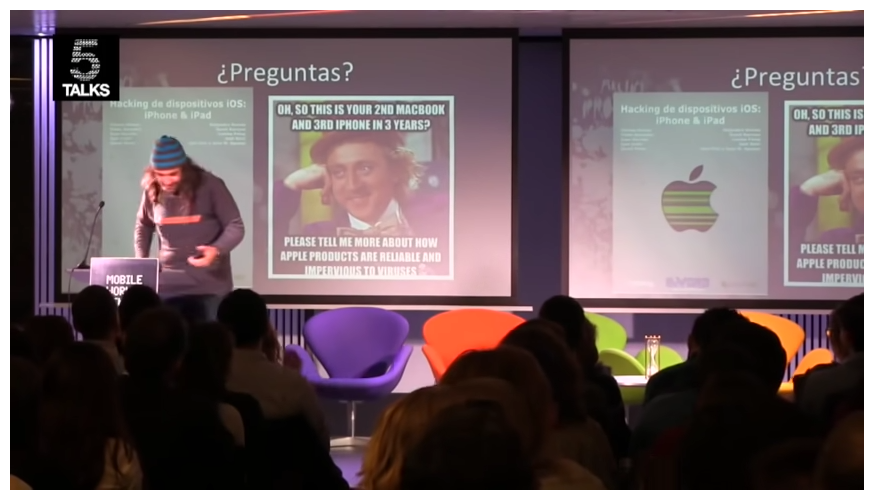
\includegraphics[scale=0.3]{figuras/chemalonso.png}
    \end{center}
\end{figure}

En todos estos casos y en muchos más, los memes se han convertido un medio para conectar con el consumidor de una manera única y efectiva.

Sin embargo, a pesar de su uso generalizado, la gestión, centralización y organización de memes sigue siendo un desafío para muchos creadores de contenido, empresas y personas.

\section{Motivación}

Como hemos comentado la creación y compartición de memes es una actividad de lo más común por lo que la falta de un sistema centralizado limita su potencial para todo tipo de usuarios. Esta falta de una solución informática específica se traduce en una pérdida de tiempo y recursos, así como en una limitación en la capacidad de generar contenido relevante y oportuno. Lo cual es una característica esencial en el mundo de los memes.

La motivación detrás de este proyecto radica en ofrecer una solución que subsane las dificultades que los usuarios encuentran a la hora de gestionar estos medios de información. Estas dificultades van desde la dificultad de encontrar memes antiguos hasta la falta de herramientas colaborativas y centralizadas. Como se puede apreciar los problemas pueden llegar a ser muy diversos y afectar a diferentes tipos de usuarios.

El proyecto `Memes para todos` aspira a proporcionar una plataforma robusta y fácil de usar que simplifique el proceso de creación, almacenamiento y distribución de memes para todo tipo de usuarios, sin importar su experiencia previa o contexto.

\section{Definición del problema}

Dentro de este marco de trabajo, para realizar una mejor de definición del problema, se han identificado una serie de personas con necesidades y objetivos específicos que junto con las historias de usuario describen los problemas que se pretenden resolver con este proyecto.

\subsection{Usuarios identificados}

    \subsubsection{María Rodríguez Espinosa (Creadora de contenido)}

    María Rodríguez Espinosa es una creadora de contenido especializada en memes. Trabaja actualmente para una famosa cadena de comida rápida. Su objetivo principal es mantener comprometida a su audiencia con contenido fresco, joven y relevante.

    \subsubsection{Juan Pérez Ruiz (CTO)}

    Juan Pérez es el CTO de una empresa de marketing digital. Como CTO, es responsable de liderar la estrategia tecnológica de la empresa y garantizar que las soluciones tecnológicas satisfagan las necesidades del negocio y de los clientes. Recientemente, el departamento de marketing le ha expresado la necesidad de un sistema centralizado para agilizar el proceso de generación y gestión de multimedia (principalmente memes).

    \subsubsection{Carlos Sánchez Ruedo (Dueño de un pequeño negocio)}

    Carlos Sánchez es el propietario de un pequeño negocio local especializado en la venta de comida rápida. Inspirado por la exitosa estrategia de KFC de posicionarse como una marca influencer en las redes sociales decide implementar una estrategia similar para promocionar su negocio y aumentar su visibilidad en línea. Sin embargo, debido a las limitaciones de recursos y la falta de experiencia tecnológica no ha dado el paso todavía.

\section{Historias de usuario}

    \subsection{María Rodríguez Espinosa (Creadora de contenido)}

    \begin{enumerate}
        \item [HU01] Como María Rodríguez, creadora de contenido de memes para KFC, necesito poder editar memes y almacenarlos.
        \item [HU02] Como María Rodríguez, creadora de contenido de memes para KFC, siempre he tenido problemas encontrando memes antiguos que he creado.
    \end{enumerate}

    \subsection{Juan Pérez Ruiz (CTO)}

        \begin{enumerate}
            \item [HU02] Como Juan Pérez, CTO, necesito que puedan colaborar varios usuarios en la creación de los memes además de administrar quién del equipo puede ver, editar o eliminar los memes.
        \end{enumerate}

    \subsection{Carlos Sánchez Ruedo (Dueño de un pequeño negocio)}

        \begin{enumerate}
            \item [HU03] Como Carlos Sánchez, dueño de un pequeño negocio, necesito un sistema que se pueda usar desde un pequeño ordenador que tengo en la tienda.
            \item [HU04] Como Carlos Sánchez, dueño de un pequeño negocio, quiero que me facilite la compartición con las redes sociales, puesto que no sé mucho de ellas y no tengo a nadie en mi equipo de marketing.
        \end{enumerate}

\section{Objetivos Iniciales}

\begin{enumerate}
    \item Diseñar una solución que sea lo más económica posible, permitiendo su instalación en servidores en la oficina o su despliegue en contenedores sin costos excesivos, lo que garantiza una mayor accesibilidad y viabilidad para organizaciones de todos los tamaños y presupuestos.
    \item Se deberá crear un sistema que comprenda una gama de clientes lo más amplia posible, ofreciendo una solución que sea capaz de adaptarse a las diferentes necesidades y preferencias de los usuarios.
    \item Se deberá garantizar la accesibilidad y facilidad de uso desarrollando una aplicación que se pueda utilizar incluso desde un ordenador de bajas prestaciones.
    \item La licencia del proyecto deberá de permitir su uso por cualquier organización o personas sin importar el fin con el que se utilice, ya sea para uso personal, educativo o empresarial.
\end{enumerate}